\chapter{積分}

%{\small 君は, 理解したことを自力で再現してみていますか? 解説や解答を
%目で追うだけになっていませんか?\\}

\section{積分の発想}
「ローマは一日にして成らず」という。何事も, 小さな変化の積み重ねが大きな変化
につながるのだ。その考え方を数学にしたのが「積分」というものである。

いま, 何かの量(ローマの都市の人口とか面積でもいい)$z$が時刻$t$とともにどう変わっていくかを
知りたいとする。最初$t=t_0$のときは$z=z(t_0)$という値であり, $t$が$t_1, t_2, \cdots, t_n$
と経つにつれ(現在を$t=t_n$とする), $z$は$z(t_1), z(t_2), \cdots, z(t_n)$という風に変化していったとしよう。
すると現在の値$z(t_n)$は, それまでの成長の積み重ねで決まる。つまり, 年々, もしくは日々の成長を, 
\begin{eqnarray}
\Delta z_1&:=&z(t_1)-z(t_0)\,\,\,\,\text{ ... $t_0$から$t_1$までの成長}\nonumber\\
\Delta z_2&:=&z(t_2)-z(t_1)\,\,\,\,\text{ ... $t_1$から$t_2$までの成長}\nonumber\\
\Delta z_3&:=&z(t_3)-z(t_2)\,\,\,\,\text{ ... $t_2$から$t_3$までの成長}\nonumber\\
\cdots\nonumber\\
\Delta z_k&:=&z(t_k)-z(t_{k-1})\,\,\,\,\text{ ... $t_{k-1}$から$t_k$までの成長}\nonumber\\\label{eq:deltaz0}\\
\cdots\nonumber\\
\Delta z_n&:=&z(t_n)-z(t_{n-1})\,\,\,\,\text{ ... $t_{n-1}$から$t_n$までの成長}\nonumber
\end{eqnarray}
とすれば, 
\begin{eqnarray}
z(t_n)&=&z(t_0)+\Delta z_1 + \Delta z_2 + \Delta z_3 + \cdots + \Delta z_n\nonumber\\
   &=&z(t_0)+\sum^{n}_{k=1}\Delta z_k\label{eq:sum_deltaz}
\end{eqnarray}
である。

さてここで, 年々や日々の成長を, もっともっと細かいステップ(分ごととか, 秒ごととか)
で考えれば, \textgt{それぞれの$\Delta z_k$は0に近づいて
無限小$dz$になり, そのかわりステップの個数$n$は無限に大きくなっていく}
(ただし$t_n$は$n$がどんなに大きくなっても「現在の時刻」に固定する)。そういう
状況で, \eref{eq:sum_deltaz}を以下のように書きあらわす:
\begin{eqnarray}
z(T)=z(t_0)+\int^{z(T)}_{z(t_0)} dz\label{eq:integral_dz}
\end{eqnarray}
ここで$t_n$を改めて$T$と置いた。
この$\int$という記号はインテグラルと呼ぶ。これは, 総和記号$\Sigma$の「極限」, 
つまり「各ステップの幅を無限小にして, ステップの数を無限大にしたときの$\Sigma$」であると
考えればよい。また, 末尾の$dz$は, ステップの幅$\Delta z_k$を0に近づける極限の無限小である。
つまり, 形式的には, 
\begin{itembox}{ステップの幅を無限小に, 数を$\infty$にする極限では}
$\quad$$\Sigma$は$\int$に変わる! 
$\quad$$\Delta z_k$は$dz$に変わる!\\
($\Delta$は$d$に変わり, $k$は消える)
\end{itembox}
のだ\footnote{計算機で積分を考えるときは, 逆に$\int$を$\Sigma$に, $dz$を$\Delta z_k$
に置き換えて考える。}。

さて, \eref{eq:sum_deltaz}や\eref{eq:integral_dz}は, 何かの量を, その微小な
変化の積み重ねで表しただけである。ところが多くの場合, 個々の微小な変化は, その変化に要した(微小な)時間
\begin{eqnarray}\Delta t_k:=t_k-t_{k-1}\end{eqnarray}
に比例すると考えてよかろう。例えば$z$がローマの大きさなら, 
2日間の変化は1日の間の変化の約2倍だろう。ただしこれが1万日くらいの長い時間になると
そんなに単純ではない。そんなに長い時間では, その間にローマの発展の勢いが
大きく変わるかもしれないから, 単純に1万日間の変化=1日の変化×1万とは言えまい。
そこで, その比例係数は, その時々で変わると考え, それを$f(t)$とし, 
$\Delta t_k$は, $f(t)$がほとんど変化しないくらい短い時間を考えれば, 
\begin{eqnarray}\Delta z_k\fallingdotseq f(t_k)\Delta t_k\label{eq:fdeltat}\end{eqnarray}
と書けるだろう。ここで気づいた人もいるだろうが, この$f(t_k)$は, 要するに
$z$を$t$の関数と見た時の微分係数(導関数)である。

すると, \eref{eq:sum_deltaz}は, 
\begin{eqnarray}
z(t_n)&\fallingdotseq&z(t_0)+\sum^{n}_{k=1}f(t_k)\Delta t_k\label{eq:sum_fdeltat}
\end{eqnarray}
となる。ここで, 先ほどやったように$t_n=T$を固定して, $\Delta t_k$が無限小になり, $n$が無限大になる極限で, 
\eref{eq:fdeltat}, \eref{eq:sum_fdeltat}
をそれぞれ以下のように書く:
\begin{eqnarray}
&&dz = f(t) \,dt\\
&&z(T)=z_0+\int^{T}_{t_0} f(t) \,dt\label{eq:WhatIsIntegral1}
\end{eqnarray}

この例のように, 一般に関数$f(x)$に, $x$の小刻みな増分$\Delta x_k=x_k-x_{k-1}$
を掛けながら足しあわせること, すなわち, 
\begin{eqnarray}
&&f(x_1)(x_1-x_0)+f(x_2)(x_2-x_1)+f(x_3)(x_3-x_2)+\nonumber\\
&&\cdots+f(x_n)(x_n-x_{n-1})\nonumber\\
&&=\sum^{n}_{k=1} f(x_k)\Delta x_k\label{eq:WhatIsIntegral15}
\end{eqnarray}
について, 最初($x_0=a$)と最後($x_n=b$)の値を固定したまま, 
ステップの幅(つまり$\Delta x_k$)をどんどん0に近づけ, $n$をどんどん増や
すときの\eref{eq:WhatIsIntegral15}の
極限を以下のように書き表す:
\begin{eqnarray}
\int_{a}^{b}f(x)\,dx\label{eq:WhatIsIntegral18}
\end{eqnarray}
これを\underline{定積分}\index{ていせきぶん@定積分}もしくは単に\underline{積分} (integral)
\index{せきぶん@積分}という。
すなわち, 
\begin{itembox}{定積分の定義}
\begin{eqnarray}
\int_{a}^{b}f(x)\,dx :=\lim_{\substack{n\rightarrow \infty\\\Delta x_k\rightarrow 0}}\sum^{n}_{k=1} f(x_k)\Delta x_k\label{eq:WhatIsIntegral2}
\end{eqnarray}
ただし, $a=x_0<x_1<x_2<\cdots<x_n=b$, $\Delta x_k=x_k-x_{k-1}$
\end{itembox}
要するに, \textgt{一定区間を無数の微小量(無限小)
に分割し, 関数にその微小量を掛けて足し合わせることが積分}である。

\begin{q}\label{q:int_define} 定積分の定義(「ただし」以下も含むよ!)
を5回書いて記憶せよ。\end{q}

積分において, 始点と終点を定め, 差分(微小量)として分割される量(変数)
のことを, \index{せきぶんへんすう@積分変数}\underline{積分変数}と呼ぶ。
\eref{eq:WhatIsIntegral1}では積分変数は$t$であり, \eref{eq:WhatIsIntegral2}では積分変数は$x$である。

積分される関数を「被積分関数」という。\eref{eq:WhatIsIntegral1}では被積分関数は$f(t)$であり, 
\eref{eq:WhatIsIntegral2}では被積分関数は$f(x)$である。\hv

\begin{freqmiss}{\small\textgt{\eref{eq:WhatIsIntegral2}の左辺を, 
\begin{eqnarray*}
\int_{a}^{b}f(x)\,\Delta x_k\,\,\,\,\text{とか,}\,\,\,\,
\int_{a}^{b}f(x)\,d x_k\,\,\,\,\text{とか,}\,\,\,\,
\int_{a}^{b}f(x_k)\,d x
\end{eqnarray*}
などと書く。} ... 積分では, 微小量$\Delta x_k$が0になる極限(無限小)を
考えているので, $\Delta$は$d$で置き換えるのです。また, それに伴って, 
和の項数は無限大になるので, 添字$k$を残すのは無意味になり, $k$を
書かないのです。}\end{freqmiss}

\begin{freqmiss}{\small\textgt{\eref{eq:WhatIsIntegral2}
の下の「ただし」以下を, $a<x_0<x_1<x_2<\cdots<x_n<b$と書く}
 ... それでは$a$から$x_0$までの間や, $x_n$から$b$までの間に
隙間ができちゃうでしょ? 「そうしたら$a$から$b$まで」を意味する$\int_a^b$が
無意味になってしまいます。}\end{freqmiss}

\begin{freqmiss}{\small\textgt{\eref{eq:WhatIsIntegral2}の左辺を, 
\begin{eqnarray*}
\int_{a}^{b}f(x)
\end{eqnarray*}
と書く。} ... $dx$を忘れちゃダメです。
積分は「\textgt{微小量を掛けて}足す」です。}\end{freqmiss}
\mv


\section{グラフと積分}\label{sect:graph_integral}
さて, \eref{eq:WhatIsIntegral2}をグラフでイメージしてみよう。
関数$y=f(x)$のグラフが\fref{fig:integral_strip}のようだとする。
話を簡単にするため, グラフは$x$軸より上にあるとする。
\eref{eq:WhatIsIntegral2}の$\sum$の中身, すなわち, 
$f(x_k)\Delta x_k$
は, この図で斜線をかけた長方形の範囲の面積である。こういう長方形を
$x=a$から$x=b$までたくさん考えると, 階段状の図形ができる。
\eref{eq:WhatIsIntegral2}のlimの内側
\begin{eqnarray}
\sum^{n}_{k=1} f(x_k)\Delta x_k\label{eq:WhatIsIntegral24}
\end{eqnarray}
は, そういう階段状の図形の面積である。
\begin{figure}[h]
    \centering
    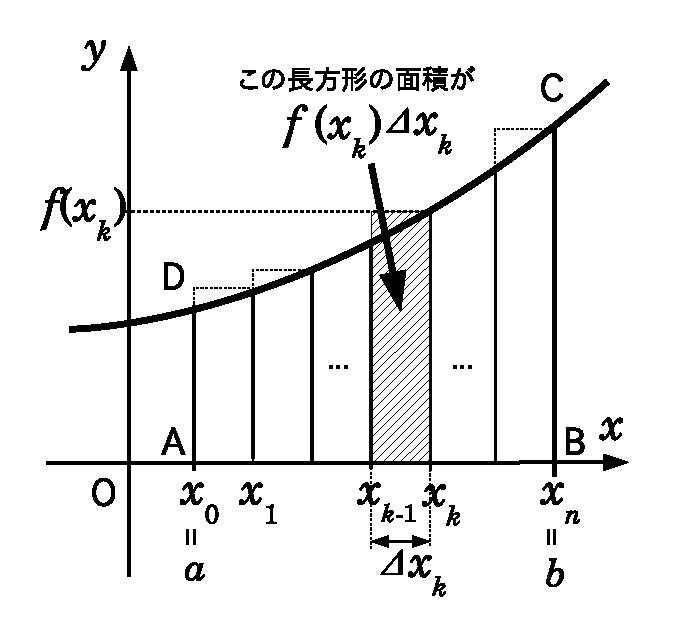
\includegraphics[width=8cm]{integral_strip.eps}
    \caption{積分のイメージ}\label{fig:integral_strip}
\end{figure}
さて, $n$を大きくし, $\Delta x_k$を0に近づけるというのは, こういう
長方形の数を限りなく増やし, それぞれの幅を限りなく狭くしていく, 
ということである。そうなると, それらを集めてできる階段状の図形は, 
図形ABCD ($x$軸上の線分ABと, 直線$x=a$上の線分AD, 直線$x=b$上の
線分BC, そして曲線$y=f(x)$上の曲がった線分CDで囲まれる図形)に
限りなく近づく。そのとき, \eref{eq:WhatIsIntegral24}は, 図形ABCDの
面積に限りなく近づいていく。つまり, \eref{eq:WhatIsIntegral2}は, 
図形ABCDの面積なのだ!

\begin{faq}{\small\textgt{てことは, 要するに「積分とはグラフの
面積」と定義してOK?} ... 今学んでいる1変数関数の積分に限れば, 
そういう性質はあります。しかし, グラフが$x$軸より下に来てしまったら, 
積分の値はマイナスになるので, 単純に「面積」とは言えません。
「グラフの面積を求めること」は, 積分概念の, ひとつの側面に過ぎ
ないのです。上述したように, 積分は関数に微小量を掛けて
足し合わせること。それが「面積を求めること」になることもあれば, 
そうならないこともあります。いずれ, 積分変数が複数個あったり, 
積分変数が複素数であったり, 被積分関数がベクトルであるような
積分も考えます。そういうとき, 「面積を求めること」という理解は
破綻しますが, 「関数に微小量を掛けて足し合わせること」という定義
は破綻しないのです (ただし, このような定義も, 「ルベーグ積分」
\index{るべーぐせきぶん@ルベーグ積分}という, より普遍性の高い
積分概念の前では破綻しますが, そのレベルの数学まで到達する
資源生はほとんどいないでしょう)。}\end{faq}

\begin{faq}{\small\textgt{「定積分の定義を述べよ」という問題で, 
「関数に微小量を掛けて足し合わせること」と書いたら不正解でした。
テキストにはそう書いてあるのに!}
... それは定義を言葉で簡略的に表現し, イメージしやすくしたものです。
\eref{eq:WhatIsIntegral2}を書かねばなりません。}\end{faq}
\mv


\section{数値積分}\label{sect:suuchisekibun}

これから具体的に関数を積分する方法を学ぶのだが, まず, 
計算機で積分するやり方を学ぼう。それを
「\underline{数値積分}」 \index{すうちせきぶん@数値積分}という。
数値積分は原理が単純で, 積分のアイデアを理解するのに
良い題材だ。また, 実際に世の中で数値積分は様々な場で使われている。
というわけで, 積分の勉強はまず計算機から入るのだ。

\begin{faq}{\small\textgt{ん? なんか同じようなセリフを\pref{sect:numdiff}
あたりで読んだような...} ... 気のせいでしょう!}\end{faq}

\eref{eq:WhatIsIntegral2}で学んだように, 
積分は, 「関数に微小量を掛けて足すこと」である:
\begin{eqnarray*}\int_{a}^{b}f(x)dx&\fallingdotseq&\sum^{n}_{k=1} f(x_k)\Delta x_k\\
&=&f(x_1)(x_1-x_0)\\
&+&f(x_2)(x_2-x_1)\\
&+&f(x_3)(x_3-x_2)\\
&+&\cdots\\
&+&f(x_n)(x_n-x_{n-1})
\end{eqnarray*}
(ただし, $x_0=a, x_n=b, \Delta x_k=x_k-x_{k-1}$)

$n$が無限に大きく, $\Delta x_k$が無限小になるときだけ, 近似等号"$\fallingdotseq$"は
等号"="になる。しかし, 実際は, $\Delta x_k$が無限小でなくても, ある程度の小ささであれば, 
これがだいたい成り立つとしてOKだろう。これが, 数値積分だ。

では表計算ソフトで数値積分してみよう。例として, 関数$f(x)=2x$を, 
$0\leq x \leq3$で数値積分してみよう。まず以下のように
$f(x)=x$の値をスプレッドシートに与える(ここでは$x$の刻みを0.1とした):\\
\begin{tabular}{|>{\columncolor[gray]{0.8}}c|c|c|c|} \hline
\rowcolor[gray]{0.8} & A & B & C \\ \hline
1 & x    &  f(x) & sekibun \\ \hline
2 & 0.0  & 0 &  \\ \hline
3 & 0.1  & 0.2 &  \\ \hline
4 & 0.2  & 0.4 &  \\ \hline
5 & 0.3  & 0.6 &  \\ \hline
$\cdots$ & $\cdots$ & $\cdots$ &  \\ \hline
32 & 3  & 6 &  \\ \hline
\end{tabular}\\
ここで右端の列(C列)に積分を計算するには, まず積分の出発の値(初期値)としてセルC2に0を書き込む。
次に, セルC3に, 「=C2+B3*(A3$-$A2)」という式を書き込む。この式でB3が$f(x_1)$に相当し, A3$-$A2が
$\Delta x_1$に相当する。

そして, セルC3の内容を, セルC4以降のC列全体にコピーペーストすれば
(ここで「相対参照」が役に立つ!), C列に0から$x$までの積分ができあがる:\\
\begin{tabular}{|>{\columncolor[gray]{0.8}}c|c|c|c|} \hline
\rowcolor[gray]{0.8} & A & B & C \\ \hline
1 & x    &  f(x) & sekibun \\ \hline
2 & 0.0  & 0 &  0\\ \hline
3 & 0.1  & 0.2 & 0.02\\ \hline
4 & 0.2  & 0.4 & 0.06 \\ \hline
5 & 0.3  & 0.6 & 0.12 \\ \hline
$\cdots$ & $\cdots$ & $\cdots$ &  \\ \hline
32 & 3  & 6 & 9.3\\ \hline
\end{tabular}\\
例えば, セルC5には, $\int_0^{0.3}2x\,dx$の値が入っているし, セルC32には
$\int_0^{3}2x\,dx$の値が入っている。もっとも, これらの値には誤差が
含まれている。刻みをもっと細かく, 例えば0.01などにしたら, もっと正確な
結果が得られる。こうして計算機で関数の積分を\textgt{近似的に}やるのが
数値積分だ。
%なお, 数値積分できるのは, 定積分だけである。不定積分は数値積分では求めることはできない。つまり, 
%定積分よりも不定積分のほうが, 一般には難しいのだ!\\

\begin{faq}{\small\textgt{セルC2に0を入れるのはなぜですか?} ... 
まだ何も足していない状態を意味します(次節で学ぶ\eref{ed_int_th4}
に相当します)。}\end{faq}

\begin{q}\label{q:int03x2} パソコンの表計算ソフトで, 関数$f(x)=2x$を, 
$0 \le x \le 3$の範囲で数値積分し, その結果を, $f(x)$とともに, 
グラフに描け。刻みは各自で適当に定めよ。回答は
\fref{fig:int03x2}のようになるはず。
\end{q}\mv

\begin{figure}[h]
    \centering
    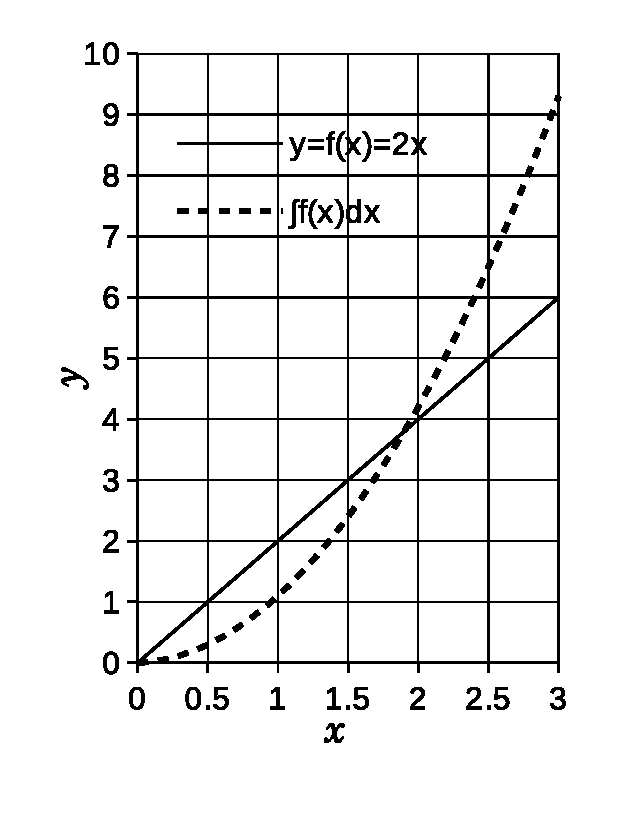
\includegraphics[width=6cm]{int03x2.eps}
    \caption{$y=2x$と, その数値積分}\label{fig:int03x2}
\end{figure}

\fref{fig:int03x2}を見ると, $y=2x$の積分のグラフ(\fref{fig:int03x2}の点線)は, 
形からして放物線みたいだ。$x=1$で$y\fallingdotseq1$, $x=2$で$y\fallingdotseq4$, 
$x=3$で$y\fallingdotseq9$だから, $y=x^2$か? 
実はそうなのだ(多少のズレは数値積分の誤差)。そして, 
$y=2x$と$y=x^2$の関係って... そうだ! 後者を微分したら前者になる!

そう, 実は, 積分と微分は逆の演算なのだ。それを感じられる問題をやってみよう。

\begin{q}\label{q:int03x2_diff} 前問の数値積分の結果を数値微分し, 
もとの関数$f(x)=2x$と値を比較せよ。ヒント: 前問題のC列を数値微分する。
例えば, セルD2に「=(C3-C2)/(A3-A2)」と打ち込む。それをセルD3からセルD31
までペーストすればよい。そしてD列をB列(もとの関数$2x$)と比べればよい。
\end{q}\mv

なんと! 数値積分を数値微分すると, もとの関数と同じになるじゃないか! 
これは偶然ではない。$f(x)$がどんな関数でも, それを積分して微分すれば, 
もとに戻るのだ。このことは, 後で理論的に確認する。

\begin{freqmiss}{\small\textgt{てことは, 要するに「積分とは微分の逆」
と定義してOK?} ... 今学んでいる1変数関数の積分に限れば, 
確かにそういう性質があります。そういうスタイルで定義される積分
を「不定積分」と言います(後で学ぶ)。しかし, 積分の概念には, 
単なる「微分の逆」では捉えきれない広がりがあります。例えば
いずれ学ぶ「面積分」や「体積分」という種類の積分は, 「微分の逆」
では定義できません。何回も言いますが, 積分は, あくまで
「関数に微小量をかけて足しあわせる」こと。「微分の逆」は, たまに
ついてくるオマケみたいなものです。}\end{freqmiss}

\begin{q}\label{q:comp_int2} 表計算ソフトで, 関数$f(x)=\cos x$を, 
$0 \le x \le 7$の範囲で数値積分せよ。また, その結果を数値微分せよ。
それらのグラフを重ねて描け。$\Delta x$は各自で適当に定めよ。回答は
\fref{fig:intcos}のようになるはず。
\end{q}\mv

\begin{figure}[h]
    \centering
    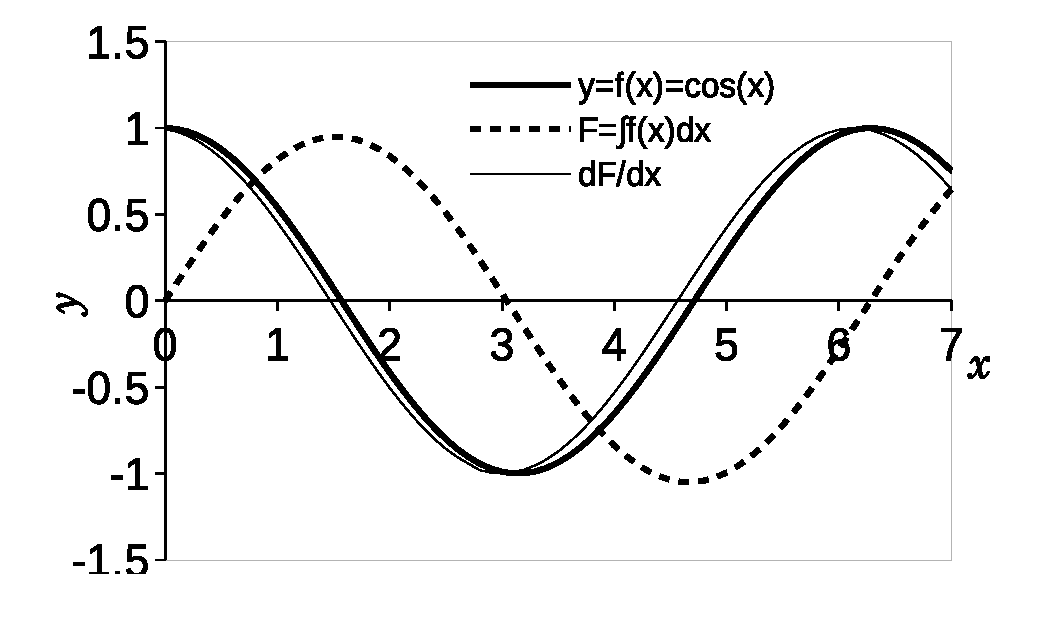
\includegraphics[width=6cm]{intcos.eps}
    \caption{$y=\cos x$ (太実線)と, その数値積分(点線), 
そしてその数値微分(細実線)。$x$の刻みは0.1。この刻みを小さくすると, 
太実線と細実線はもっと近くなる。}\label{fig:intcos}
\end{figure}


\section{積分の公式}\label{sect:integral_formula}


実際に関数を積分するときは, 積分の定義\eref{eq:WhatIsIntegral2}に
遡ってやることは少ない。複雑な関数の場合は前節でやったように数値積分を使うし, 
そうでなければ, 以下に示すような, いくつかの便利な定理(公式)を活用して
ちゃっちゃとやってしまうのだ。

\begin{faq}{\small\textgt{ん? なんか同じようなセリフを\pref{sect:diff_formula}
あたりで読んだような...} ... 気のせいでしょう!}\end{faq}

以下, $a, b, c$は実数の定数, $f(x), g(x)$を, 任意の(積分可能な)
関数とする\footnote{詳しくは説明しないが, 世の中には積分できない関数も存在する。例えば
次式のような積分はできない($\infty$に発散する): 
\begin{eqnarray*}\int_{0}^{1}\frac{1}{x}\,dx\end{eqnarray*}
}。また, 以後, 本章で出てくる変数や定数は全て実数とする(虚数は考えない)。
\mv

\begin{itembox}{積分の公式1: 足し算はバラせる}
\begin{eqnarray}
\int_{a}^{b}\{f(x)+g(x)\}\, dx=\int_{a}^{b}f(x)\, dx+\int_{a}^{b}g(x)\, dx\nonumber\\
\label{eq:int_baraseru}\end{eqnarray}
\end{itembox}
証明:
\begin{eqnarray*}
&&\int_{a}^{b}\{f(x)+g(x)\}\, dx \fallingdotseq \sum_{k=1}^n \{f(x_k)+g(x_k)\}\, \Delta x_k\\
&&=\sum_{k=1}^n f(x_k) \Delta x_k + \sum_{k=1}^n g(x_k) \Delta x_k\\
&&\fallingdotseq \int_{a}^{b}f(x)\, dx + \int_{a}^{b}g(x)\, dx
\end{eqnarray*}
1行目から2行目にかけてP.\pageref{eq:sum_linear1}の\eref{eq:sum_linear1}を使った。\qed
注: ここでの"$\fallingdotseq$"は, $\Delta x_k$を無限小
に, $n$を無限大にする極限では等号"="になる。以下, 同様。\hv

\begin{freqmiss}{\small\textgt{\eref{eq:int_baraseru}の左辺を
\begin{eqnarray*}
\int_{a}^{b}f(x)+g(x)\, dx
\end{eqnarray*}
と書く。} ... カッコを忘れちゃダメです。理由は, 上の証明を見ればわかります。
カッコがないと, $f(x)$には微小量がかかりません($dx$が$g(x)$だけに
かかる)。}\end{freqmiss}

\begin{itembox}{積分の公式2: 定数倍は前に出せる}
\begin{eqnarray}
\int_{a}^{b}cf(x)\, dx=c\int_{a}^{b}f(x)\, dx
\end{eqnarray}
\end{itembox}
証明:
\begin{eqnarray*}
\int_{a}^{b}cf(x)\, dx &\fallingdotseq& \sum_{k=1}^n cf(x_k)\, \Delta x_k\\
&=&c\sum_{k=1}^n f(x_k)\,\Delta x_k \fallingdotseq c\int_{a}^{b}f(x)\, dx
\end{eqnarray*}
1行目から2行目にかけてP.\pageref{eq:sum_linear2}の\eref{eq:sum_linear2}を使った。\qed

\begin{itembox}{積分の公式3: 積分区間は分割できる}
\begin{eqnarray}
\int_{a}^{b}f(x)\, dx+\int_{b}^{c}f(x)\, dx=\int_{a}^{c}f(x)\, dx\,\,\,\,\,\,\,\,\,\,\,\,\,\,\,\,\,\label{eq:sekibun_koshiki3}
\end{eqnarray}
\end{itembox}
証明: $a$から$c$までの区間を$m$個に分割し, 途中, $n$個めの分割($n\leq m$とする)の右端
が$b$になるようにする。つまり$x_0=a$, $x_n=b$, $x_m=c$である。$m, n$が十分に大きければ, 
積分の定義から, 
\begin{eqnarray}
&&\int_{a}^{b}f(x)\, dx \fallingdotseq \sum_{k=1}^n f(x_k)\Delta x_k\\
&&\int_{b}^{c}f(x)\, dx \fallingdotseq \sum_{k=n+1}^m f(x_k)\Delta x_k
\end{eqnarray}
である。このとき, 右辺どうしを足し合わせると, 
\begin{eqnarray*}
\sum_{k=1}^n f(x_k)\Delta x_k + \sum_{k=n+1}^m f(x_k)\Delta x_k = \sum_{k=1}^m f(x_k)\Delta x_k
\end{eqnarray*}
となる。$x_0=a$, $x_n=b$, $x_m=c$を固定したまま, $n$と$m$を限りなく大きくして$\Delta x_k$を
限りなく小さくすれば, この式は, 積分の定義から
\begin{eqnarray*}
\int_{a}^{b} f(x)\, dx + \int_{b}^{c} f(x)\, dx = \int_{a}^{c} f(x)\, dx
\end{eqnarray*}
\qed
\vspace{0.3cm}

さて, 積分の定義によると, $\int_{a}^{b}f(x)\,dx$は, 
$a<b$が前提だった(\eref{eq:WhatIsIntegral2}の「ただし」以下を見よ)。
これを, $a\geq b$の場合にも拡張しよう。それには, ここまで証明してきた
公式が, $a\geq b$の場合にも成り立つように, つじつまを合わせればよい。
まずは$a=b$の場合。積分の公式3で, $b=c=a$とすれば, 
\begin{eqnarray*}
\int_{a}^{a}f(x)\,dx +\, \int_{a}^{a}f(x)\, dx = \int_{a}^{a}f(x)\, dx
\end{eqnarray*}
右辺を左辺に移項すれば, 
\begin{eqnarray*}
\int_{a}^{a}f(x)\, dx=0
\end{eqnarray*}
よって, 以下のように約束しよう:
\begin{itembox}{積分の公式4: 始点=終点なら積分は0}
\begin{eqnarray}
\int_{a}^{a}f(x)\, dx=0\label{ed_int_th4}
\end{eqnarray}
\end{itembox}
\vspace{0.3cm}

次に, $a>b$の場合。積分の公式3で, $c=a$とすれば, 
\begin{eqnarray}
\int_{a}^{b}f(x)\, dx+\int_{b}^{a}f(x)\, dx=\int_{a}^{a}f(x)\, dx
\end{eqnarray}
ここで積分の公式4より, この右辺は0。従って, 以下のように約束しよう:
\begin{itembox}{積分の公式5: 積分区間を逆転すると正負も逆転}
\begin{eqnarray}
\int_{a}^{b}f(x)\,dx=-\int_{b}^{a}f(x)\,dx\label{eq:sekibun_koshiki5}
\end{eqnarray}
\end{itembox}
\vspace{0.3cm}

次に, 積分と微分の関係を調べていこう。

\begin{itembox}{積分の公式6: 微小区間の積分は単なる掛け算}
$f(x)$を連続関数とする。$h$が微小量であれば, つまり$a \le x \le a+h$の範囲で$f(x)$がほとんど変化しなければ, 
\begin{eqnarray}
\int_{a}^{a+h}f(x)\, dx\fallingdotseq f(a)h
\end{eqnarray}
\end{itembox}
証明: $x_0=a, x_n=a+h$として, 積分の定義より, 
\begin{eqnarray}
\int_{a}^{a+h}f(x)\, dx\fallingdotseq \sum_{k=1}^n f(x_k)\Delta x_k
\end{eqnarray}
とできる。$x_k$を$a \le x_k \le a+h$の範囲に限定すれば, $h$は微小量であるという
前提から, $f(x_k)\fallingdotseq f(x_0)=f(a)$。従って, 
\begin{eqnarray*}
\sum_{k=1}^n f(x_k)\Delta x_k \fallingdotseq \sum_{k=1}^n f(a)\Delta x_k = f(a)\sum_{k=1}^n \Delta x_k
\end{eqnarray*}
ここで, $\Delta x_k$は, $a$から$a+h$までの範囲を$n$個の区間に刻んだものなので, その総和は$h$となる。従って, 
\begin{eqnarray}
f(a)\sum_{k=1}^n \Delta x_k=f(a)h
\end{eqnarray}
従って, 与式が成り立つ。\qed
\vv

\begin{itembox}{積分の公式7: 積分の微分は元の関数}
$f(x)$を連続関数とし, $a$を定数とする。
\begin{eqnarray}
\frac{d}{dx}\int_{a}^{x}f(t)\, dt=f(x)\label{eq:sekibun_koshiki7}
\end{eqnarray}
\end{itembox}
証明: $a$を任意の定数とし, 
\begin{eqnarray}F(x):=\int_{a}^{x}f(t)\, dt\end{eqnarray}
とおくと, 
\begin{eqnarray}F(x+dx)=\int_{a}^{x+dx}f(t)\, dt\end{eqnarray}
となる($dx$は無限小)。ここで積分の公式3から, 
\begin{eqnarray}
F(x+dx)&=&\int_{a}^{x}f(t)\, dt+\int_{x}^{x+dx}f(t)\, dt\nonumber\\
              &=&F(x)+\int_{x}^{x+dx}f(t)\, dt\label{eq:intform7-}
\end{eqnarray}
$dx$は微小量なので積分の公式6より, 
\begin{eqnarray}
\int_{x}^{x+dx}f(t)\, dt = f(x) dx
\end{eqnarray}
となる($dx$は無限小なので$\fallingdotseq$が$=$になった)。従って, \eref{eq:intform7-}右辺は, 
\begin{eqnarray*}
F(x)+\int_{x}^{x+dx}f(t)\, dt = F(x)+ f(x)dx
\end{eqnarray*}
となる。従って, \eref{eq:intform7-}は,
\begin{eqnarray}
F(x+dx)= F(x)+ f(x) dx
\end{eqnarray}
となる。従って, 導関数の定義\eref{eq:define_dif}(P.\pageref{eq:define_dif})より, 
\begin{eqnarray*}
\frac{d}{dx}F(x)=f(x)
\end{eqnarray*}
\qed
この公式7は, 問\ref{q:int03x2_diff}で見たことを裏付けるものだ。\\

\begin{itembox}{積分の公式8: 微分の積分は元の関数}
$f(x)$を微分可能な関数とする。
\begin{eqnarray}
\int_{a}^{x}\frac{d}{dt}f(t)\, dt=f(x)-f(a)\label{eq:integ_formula8}
\end{eqnarray}
\end{itembox}
証明: まず, 積分の定義より, 
\begin{eqnarray}
\int_{a}^{x}\frac{d}{dt}f(t)\, dt\fallingdotseq\sum_{k=1}^{n}f'(t_k)\Delta t_k\label{eq:int_8_0}
\end{eqnarray}
である。ここで$t_0=a$, $t_n=x$, $\Delta t_k=t_k-t_{k-1}$である。$\Delta t_k$が微小なとき, 微分係数の定義から, 
\begin{eqnarray}f(t_k) \fallingdotseq f(t_{k-1})+f'(t_k)\Delta t_k\end{eqnarray}
が成り立つ。すなわち, 
\begin{eqnarray}f'(t_k)\Delta t_k\fallingdotseq f(t_k)-f(t_{k-1})\end{eqnarray}
である。従って, \eref{eq:int_8_0}右辺は, 
\begin{eqnarray}
\sum_{k=1}^{n}\{f(t_k)-f(t_{k-1})\}
=&f(t_1)&-f(t_0)\nonumber\\
+&f(t_2)&-f(t_1)\nonumber\\
+&\cdots\nonumber\\
+&f(t_{n-1})&-f(t_{n-2})\nonumber\\
+&f(t_n)&-f(t_{n-1})\label{eq:int_8_1}
\end{eqnarray}
となる。この式は, 前後の行どうしで打ち消し合って, 最初と最後, つまり$f(t_0)$と$f(t_n)$
しか残らず, 結局, $f(t_n)-f(t_0)$, すなわち$f(x)-f(a)$になる。\qed
\mv

公式7, 8を\underline{解析学の基本定理}\index{かいせきがくのきほんていり@解析学の基本定理}
と呼ぶ。ある関数をどこかから$x$まで積分して$x$で微分すれば, もとの関数になってしまう
(公式7)し, ある関数を微分して積分しても, もとの関数に戻ってしまう(公式8)。
つまり, 微分と積分は, 互いに逆の操作である (あくまで今学んでいる範囲では)。
\vv




\section{原始関数と不定積分}

ここで話はちょっと変わり, 「原始関数」と「不定積分」というものを学ぼう。
この話は, 後で関数の積分を実際に計算する方法を学ぶための準備である。

ある関数$F(x)$を微分したら関数$f(x)$になるようなとき, すなわち
\begin{eqnarray}
\frac{d}{dx}F(x)=f(x)\label{eq:def_genshikansu}
\end{eqnarray}
となるとき, $F(x)$を\underline{$f(x)$の原始関数} 
\index{げんしかんすう@原始関数}と呼ぶ(定義)。
もちろん, このとき, $f(x)$は$F(x)$の導関数である。従って, 
原始関数は導関数の対義語である。

\begin{exmpl}\label{exmpl:futeisekibun_2x_xx}
\begin{eqnarray}\frac{d}{dx}\,x^2=2x\end{eqnarray}
従って, $x^2$は$2x$の原始関数である。(例おわり)\end{exmpl}

\begin{freqmiss}{\small\textgt{原始関数を原子関数と書いてしまう。}}\end{freqmiss}

\begin{freqmiss}{\small\textgt{「$F(x)$を微分して$f(x)$になるとき
$F(x)$を原始関数と呼ぶ」}... そう書いたら「$F(x)$を\underline{$f(x)$の}原始関数と呼ぶ」
と言わねばなりません。原始関数は単体で成立する概念ではありませんから。}\end{freqmiss}

ある関数$f(x)$の原始関数$F(x)$を一般的に求めることを\underline{不定積分}
\index{ふていせきぶん@不定積分}とよび, 以下のように書き表す:
\begin{eqnarray}
\int_{}^{} f(x)\, dx\label{eq:def_futeisekibun0}
\end{eqnarray}
\eref{eq:def_futeisekibun0}は\eref{eq:WhatIsIntegral2}の左辺と
よく似た記号を使っているし, 「不定」という語がついているものの「積分」
という用語も使っている。しかし, 不定積分は「原始関数を求めること」
であり, \eref{eq:WhatIsIntegral2}で定義される「積分」とは
別物なのだ。\eref{eq:WhatIsIntegral2}の積分を\underline{定積分}
\index{ていせきぶん@定積分}とも呼ぶのは, この「不定積分」との区別を
明示するためである。とは言うものの, 後で学ぶように, 定積分と不定積分の
間には実は密接な関係がある。だから, 慣習的には, 不定積分も定積分も
まとめて「積分」と呼ぶことも多い。\hv

\begin{freqmiss}{\small\textgt{「$F(x)=\int f(x)dx$となる$F(x)$を$f(x)$の原始関数と呼ぶ」}
... それは不定積分の式ですね。不定積分は「原始関数を求めること」です。
この「定義」を言い換えると, 「$f(x)$の原始関数を求めたら$F(x)$になるとき, 
$F(x)$を$f(x)$の原始関数という」となります。定義として変でしょ?}\end{freqmiss}

さて, 定数は微分したら0になるので, ある関数の原始関数に, 定数を足したり
引いたりしたものも原始関数になる。

\begin{exmpl}\label{exmpl:futeisekibun_2x_xx_2}
\begin{eqnarray}\frac{d}{dx}\,(x^2+3)=2x\end{eqnarray}
従って, $x^2+3$も$2x$の原始関数である。(例おわり)\end{exmpl}

また, ある関数$f(x)$に2つの原始関数
$F(x), G(x)$があったとすると, その差$F(x)-G(x)$を微分すれば, 
\begin{eqnarray}
\frac{d}{dx}\{F(x)-G(x)\}&=&F'(x)-G'(x)\\
&=&f(x)-f(x)=0
\end{eqnarray}
となるので, $F(x)-G(x)$は定数である (微分して恒等的に0になる関数
は定数関数しかないので)。つまり, 

\begin{itembox}{積分の公式9: 原始関数の不定性}
関数$f(x)$の原始関数が$F(x)$であるとき, それに任意の定数$C$を足した関数$F(x)+C$も, 
$f(x)$の原始関数である。また, 逆に, $f(x)$の任意の2つの原始関数の差は, 定数である。
\end{itembox}

従って, 原始関数は, 定数の足し引きのぶんだけ, 不確定である。その不確定な定数のこと
を\underline{積分定数} \index{せきぶんていすう@積分定数}と呼び, 通常は$C$と書く。

不定積分は原始関数を\underline{一般的に}求めることなので, 答えには
常に積分定数$C$をつけねばならない。

\begin{exmpl}\label{exmpl:futeisekibun_2x_xx_3}
$2x$の原始関数は, 一般的に, $x^2+C$と書ける($C$は積分定数)。すなわち, 
\begin{eqnarray}
\int_{}^{} 2x\, dx=x^2+C
\end{eqnarray}
(例おわり)
\end{exmpl}

\begin{freqmiss}{\small\textgt{不定積分して, 積分定数をつけ忘れる。}}\end{freqmiss}

以後しばらく, 不定積分において重要な公式をいくつか示す。これらの多くは, 
定積分でも似たようなものがあったことに君は気づくだろう:\hv

\begin{itembox}{積分の公式10: $x^a$の不定積分}
$a$を$-1$以外の定数とすると, 
\begin{eqnarray}
\int_{}^{} x^a \,dx=\frac{1}{a+1}x^{a+1}+C\label{eq:futeisekibun_koshiki10}
\end{eqnarray}
\end{itembox}
証明:微分で学んだように, $a \ne -1$ならば, 実際, 
\begin{eqnarray}\frac{d}{dx}\Bigl(\frac{1}{a+1}x^{a+1}\Bigr)=x^a\end{eqnarray}
\qed

\begin{q}\label{q:int_0} 上の公式を利用して以下の不定積分を求めよ。
\begin{edaenumerate}<3>
\item \begin{eqnarray*}\int_{}^{} x^2\, dx\end{eqnarray*}
\item \begin{eqnarray*}\int_{}^{} \frac{1}{x^2}\, dx\end{eqnarray*}
\item \begin{eqnarray*}\int_{}^{}\, dx\end{eqnarray*}
\end{edaenumerate}\end{q}
\vspace{0.3cm}

また, 積分の公式1, 2は, 不定積分についても成り立つ。というのも, もし$f(x), g(x)$の
原始関数がそれぞれ$F(x), G(x)$ならば, 
\begin{eqnarray*}
&&(F(x)+G(x))'=F'(x)+G'(x)=f(x)+g(x)\\
&&(aF(x))'=aF'(x)=af(x)
\end{eqnarray*}
なので, $F(x)+G(x)$は$f(x)+g(x)$の原始関数であり, $aF(x)$は$af(x)$の原始関数である。従って, 

\begin{itembox}{積分の公式11: 線型性}
\begin{eqnarray}
&&\int_{}^{} \bigl\{f(x)+g(x)\bigr\}\, dx=\int_{}^{} f(x)\, dx + \int_{}^{} g(x)\, dx\nonumber\\
\label{eq:futeisekibun_koshiki11_2}\\
&&\int_{}^{} af(x)\, dx=a\int_{}^{} f(x)\, dx
\end{eqnarray}
ただし, 右辺に任意の定数(積分定数)がついてもかまわない。
\end{itembox}

\begin{freqmiss}{\small\textgt{\eref{eq:futeisekibun_koshiki11_2}の左辺を, $\int_{}^{} f(x)+g(x)\, dx$
と書いてしまう} ... これはダメ。定積分でも不定積分でも意味的・形式的には, 
$dx$は$f(x)+g(x)$全体にかかる乗算なので, $f(x)+g(x)$は括弧( )に入れなければ
いけません。}\end{freqmiss}\mv

\begin{exmpl} 以下の不定積分を求めてみよう:
\begin{eqnarray}\int_{}^{} (2+3x)\, dx\label{eq:exmpl_futeisekibun1}\end{eqnarray}
積分の公式11より, 与式は, 
\begin{eqnarray}
\int_{}^{} 2\,dx+\int_{}^{} 3x\,dx=2\int_{}^{} dx+3\int_{}^{} x\,dx\label{eq:exmpl_futeisekibun20_01}
\end{eqnarray}
となる。右辺の各項に積分の公式10, つまり\eref{eq:futeisekibun_koshiki10}を使えば, 与式は, 
\begin{eqnarray}
=2(x+C_1)+3\Bigl(\frac{x^2}{2}+C_2\Bigr)\label{eq:exmpl_futeisekibun20_02}
\end{eqnarray}
となる。ここで$C_1$, $C_2$は, それぞれ$\int_{}^{} dx$と$\int_{}^{} x\,dx$から
生じる積分定数であり, それぞれ任意の実数である。この式を整理すると, 
\begin{eqnarray}
=2x+\frac{3x^2}{2}+2C_1+3C_2\label{eq:exmpl_futeisekibun20}
\end{eqnarray}
となる。ところが, $C_1$, $C_2$は任意の実数なので, $2C_1+3C_2$も任意の実数である。
従って$2C_1+3C_2$を改めて$C$とおけば, 与式は
\begin{eqnarray}
=2x+\frac{3x^2}{2}+C\label{eq:exmpl_futeisekibun2}
\end{eqnarray}
となる。この例では説明のために積分定数のことを念入りに書いたが, 結局最後には
積分定数は一つにまとまってしまった。従って, いくつかの関数の定数倍や和で
あらわされる関数の不定積分は, それぞれの項を, 積分定数をいったん忘れて不定積分し, 
最後に全体でひとつの積分定数をつけたせばよい。つまり, \eref{eq:exmpl_futeisekibun1}
という問に対して, \eref{eq:exmpl_futeisekibun20_01}, \eref{eq:exmpl_futeisekibun20_02}, 
\eref{eq:exmpl_futeisekibun20}を省略していきなり\eref{eq:exmpl_futeisekibun2}を
答えてよい。(例おわり)
\end{exmpl}
\mv

ここで注意: 不定積分の結果は元の関数の原始関数
のはずだから, 結果を微分したら元の関数に戻るはず。だから, 不定積分
の結果に自信が持てない場合は, \textgt{その結果を微分して元の関数に戻るかどうか
確かめる}とよい(ほとんどの場合, 関数は不定積分するより微分する方が計算は
簡単である)。不定積分に慣れていない人には, 特にそのことを\textgt{強く勧めておく}。\hv

\begin{q}\label{q:int_2} 以下の不定積分を求めよ。得られた原始関数を微分し, 被積分関数に
戻ることを確認せよ。
\begin{eqnarray}\int_{}^{} (1+x+x^2)\, dx\end{eqnarray}
\end{q}
\mv

ところで, $x^a$の不定積分に関する公式10は, $a=-1$のとき, つまり$1/x$については使えない。なぜなら, このとき$a+1=0$
となって「0での割り算」が発生してしまうからである。ここで, 自然対数の微分, すなわち\peref{eq:logdif}を思いだそう:
\begin{eqnarray}
(\ln x)'=\frac{1}{x}
\end{eqnarray}
これを使えば, $1/x$の不定積分は以下のようになりそうな気がする
\footnote{\begin{eqnarray*}\int \frac{1}{x}\,dx\,\,\,\text{を}\,\,\,\int \frac{dx}{x}\,\,\,\text{と書く。}\end{eqnarray*}}:\\
\begin{eqnarray}\int_{}^{} \frac{dx}{x}=\ln x+C\end{eqnarray}
ただし, $\ln x$という関数は, $0<x$でしか成立しない。しかし, $1/x$という関数は, 
$x<0$でも成立する。では, $x<0$も含めた$1/x$の不定積分はどうなるだろう? 
答えは, $\ln (-x)+C$である(この場合, $x<0$だから, $\ln$の内側の$-x$は正である)。
実際, これを微分してみると, 合成関数の微分より, 
\begin{eqnarray}
\{\ln (-x)\}'=(-x)'\frac{1}{-x}=\frac{1}{x}
\end{eqnarray}
となり, 確かに$1/x$になる。つまり, 
\begin{eqnarray}
&&\text{$0<x$のとき, }\int \frac{dx}{x}=\ln x+C\\
&&\text{$x<0$のとき, }\int \frac{dx}{x}=\ln (-x)+C
\end{eqnarray}
となる。いずれの場合も, 右辺の$\ln$の内側は正なので, いっそ統一的に$|x|$
と書いてしまおう。要するに, $x$が正だろうが負だろうが, 次式が成り立つ:

\begin{itembox}{積分の公式12: $1/x$の不定積分}
\begin{eqnarray}
\int \frac{dx}{x}=\ln |x|+C\label{eq:int_theorem12}
\end{eqnarray}
\end{itembox}

\begin{faq}{\small\textgt{なんで絶対値が出てきたのか, 不思議です}
 ... 似たような話が, 問\ref{q:exp_logdif0}(3)で出てきたの, 覚えてますか? }\end{faq}

\begin{freqmiss}{\small\textgt{$1/x$の不定積分で, lnの中の絶対値記号
を付け忘れる} ... これは毎年, 多くの資源生を泣かせるミスです (後で「微分方程式」
を学ぶときに痛い目に会うのです)。}\end{freqmiss}

\begin{faq}{\small\textgt{$1/x$の不定積分は$x^0$で1ではないのですか?}
 ... \eref{eq:futeisekibun_koshiki10}で, $a=-1$のときですか? 
あそこには「$a$を$-1$以外の定数とする」と書いてあったでしょ? それに, 
もしも無理やり$a=-1$としたら, 
\begin{eqnarray*}
\int_{}^{} x^{-1} \,dx&=&\frac{1}{-1+1}x^{-1+1}+C\\
&=&\frac{1}{0}x^{0}+C=\frac{1}{0}+C\quad\text{(これは間違い)}
\end{eqnarray*}
のように, 「0での割り算」が出てきて, うまくいかないのです。
}\end{faq}

農学や環境科学などの応用分野では, この公式12は, 極めて重要である。というのも, 様々な現象
を微分方程式というツールで記述して解析しようとするとき, この形の不定積分が, 
頻繁にあらわれるからである。詳しくは第\ref{chapt:calculus_app}章で学ぼう。\hv

指数関数は, 微分しても指数関数だから, 不定積分も簡単である:

\begin{itembox}{積分の公式13: 指数関数の不定積分}
\begin{eqnarray}
\int_{}^{} \exp x \,dx=\exp x+C
\end{eqnarray}
\end{itembox}

ところで, 関数$f(x)$の原始関数が$F(x)$であるとき, $F(ax+b)$を$x$
で微分すると($a, b$は定数とする), $af(ax+b)$となる。従って, 
\begin{eqnarray}f(ax+b)\text{の原始関数は,}\,\, F(ax+b)/a\label{eq:int_gousei_ax_b}\end{eqnarray}
となる。
\begin{exmpl} \eref{eq:int_gousei_ax_b}を使うと, 
\begin{eqnarray}
\int_{}^{} (3x+1)^4\, dx&=&\frac{1}{3\times5}(3x+1)^{4+1}+C\\
                        &=&\frac{(3x+1)^5}{15}+C
\end{eqnarray}
(例おわり)\end{exmpl}

注: \eref{eq:int_gousei_ax_b}は「合成関数の微分」を逆にしたような
公式だが, あくまで$f(\,\,)$の中が$ax+b$という形のときにしか使えない。

\begin{freqmiss}{\small 以下のような誤りをする人が多い:
\begin{eqnarray*}
\int_{}^{} \frac{dx}{1+x^2}=\frac{1}{2x}\ln|1+x^2|+C\,\,\,\,\text{これは間違い!}
\end{eqnarray*}
右辺を$x$で微分すると決して左辺には一致しない。
この積分は, 後に問\ref{q:int_chikan2}で学ぶ。}\end{freqmiss}

今まで学んだ公式を組み合わせれば, 以下のような不定積分ができる。それぞれ, 右辺を微分して確認せよ。 

\begin{exmpl}
\begin{eqnarray}
&&\int_{}^{} \frac{dx}{x-1}=\ln |x-1|+C\\
&&\int_{}^{} \frac{dx}{(2x+1)^2}=-\frac{1}{2(2x+1)}+C\\
&&\int_{}^{} \exp 2x \,dx=\frac{\exp 2x}{2}+C
\end{eqnarray}
(例おわり)\end{exmpl}
\mv

\begin{q}\label{q:int_4} 以下の不定積分を求めよ。得られた原始関数を微分し, 
被積分関数に戻ることを確認せよ。
\begin{edaenumerate}
\item \begin{eqnarray*}\int_{}^{} (2x+1)^3\, dx\end{eqnarray*}
\item \begin{eqnarray*}\int_{}^{} \frac{dx}{x+1}\end{eqnarray*}
\item \begin{eqnarray*}\int_{}^{} \frac{dx}{1-x}\end{eqnarray*}
\item \begin{eqnarray*}\int_{}^{} \exp(-x)\, dx\end{eqnarray*}
\item \begin{eqnarray*}\int_{}^{} \exp(x+1)\, dx\end{eqnarray*}
\end{edaenumerate}\end{q}

\begin{freqmiss}{\small\textgt{この問題の(3)を, $\ln|1-x|+C$と答えてしまう}
... これも毎年, 多くの資源生を泣かせるミスです。
これを微分すると, $-1/(1-x)$になってしまう! よくわからない, という人は, 
問\ref{q:exp_logdif0}(6)を復習しよう。}\end{freqmiss}
\mv

こんどは三角関数の不定積分を考えよう。\pref{eq:diff_sinx}の
\eref{eq:diff_sinx}, \eref{eq:diff_cosx}より, 
$(\sin x)'=\cos x$, $(\cos x)'=-\sin x$だから, 

\begin{itembox}{積分の公式14: 三角関数の不定積分}
\begin{eqnarray}
&&\int_{}^{} \cos x \,dx=\sin x+C\\
&&\int_{}^{} \sin x \,dx=-\cos x+C
\end{eqnarray}
\end{itembox}
となることはすぐわかる。
$\sin x$や$\cos x$の累乗や積を含むような関数は, 倍角公式などを使って
シンプルな形に変形してから不定積分する。

\begin{exmpl}\label{ex:intsinxcosx}
\begin{eqnarray*}
\int_{}^{} \cos x \sin x\,dx=\int_{}^{} \frac{\sin 2x}{2}\, dx=-\frac{\cos 2x}{4}+C
\end{eqnarray*}
ここで, \pref{eq:sin2a}の\eref{eq:sin2a}を使った。ちなみにこの不定積分は, 
後で\pref{q:int_chikan0}問\ref{q:int_chikan0}で学ぶように, 「置換積分」という方法でも可能。 (例おわり)\end{exmpl}
\vspace{0.1cm}

\begin{exmpl}
\begin{eqnarray*}
\int_{}^{} \cos^2 x \,dx=\int_{}^{} \frac{1+\cos 2x}{2}\, dx=\frac{x}{2}+\frac{\sin 2x}{4}+C
\end{eqnarray*}
ここで, \pref{eq:cos_pow2}の\eref{eq:cos_pow2}を使った。
(例おわり)\end{exmpl}
\vspace{0.1cm}

\begin{exmpl}
\begin{eqnarray*}
\int_{}^{} \sin^2 x \,dx=\int_{}^{} \frac{1-\cos 2x}{2}\, dx=\frac{x}{2}-\frac{\sin 2x}{4}+C
\end{eqnarray*}
ここで, \pref{eq:sin_pow2}の\eref{eq:sin_pow2}を使った。
(例おわり)\end{exmpl}

以上のような不定積分は, 勘と慣れがあれば, なんとかできるだろう。しかし, 一般に, 
どんな関数でもきれいに不定積分できるわけではない。ちょっと複雑な関数になると, その
不定積分は不可能になるか, できても職人芸になる。不定積分できるのは, 
被積分関数が単純でラッキーな場合だけなのだ。

例えば, $\exp(x)$の不定積分は簡単だが, P.\pageref{eq:Gauss_func}で学んだ
ガウス関数$\exp(-x^2)$\index{がうすかんすう@ガウス関数}
の不定積分は, これまで学んだ数学では不可能である (ガンマ関数という, 
君には未知の数学が必要)。

定積分や不定積分も含めて, 一般に, 問題を, 論理的に厳密な式変形によって身近な
関数(多項式や三角関数, 指数関数, 対数関数など)の組み合わせとして解くことを, 
\underline{解析的に解く} \index{かいせきてきにとく@解析的に解く}という。
上で述べたのは, 「不定積分を解析的にできるのはラッキーなときだけ」ということである。

では解析的に解けない問題はどうするか? 数値積分だ! コンピューターにやらせるのだ!
しかし数値積分には, 誤差とかいろいろ問題があるので, 解析的に解けるに
越したことはない。というわけで, 不定積分を解析的にやる練習をもう少しやろう。
\vv



\section{部分分数展開}\index{ぶぶんぶんすうてんかい@部分分数展開}
\begin{exmpl}\label{ex:bubunsekibun1} 以下の不定積分を考える:
\begin{eqnarray}
\int_{}^{} \frac{dx}{x^2+x}
\end{eqnarray}
被積分関数が, 2次式の逆数になっているので, このままでは不定積分できない。
そこで, 以下のように変形する:
\begin{eqnarray}
&&=\int_{}^{} \frac{dx}{x(x+1)}\label{eq:bubunsekibun3}\\
&&=\int_{}^{} \Bigl(\frac{1}{x}-\frac{1}{x+1}\Bigr)\label{eq:bubunsekibun4}\,dx\\
&&=\int_{}^{} \frac{dx}{x}-\int_{}^{}\frac{dx}{x+1}
\end{eqnarray}
こうすると, 被積分関数は, 1次式の逆数になる。1次式の逆数は, $1/x$を
変形したものだから, $1/x$の不定積分を応用することができる。すなわち, 
\begin{eqnarray}
=\ln |x| - \ln |x+1| + C
\end{eqnarray}
となる(積分定数を$C$とする)。ここで終えてもよいが, 普通は, $\ln$をひとまとめにして, 
\begin{eqnarray}
=\ln \Bigl|\frac{x}{x+1}\Bigr| + C
\end{eqnarray}
とする。(例おわり)
\end{exmpl}

例\ref{ex:bubunsekibun1}の\eref{eq:bubunsekibun3}から\eref{eq:bubunsekibun4}の変形
のように, $x$の多項式が分数の分母になっているような関数は, $x$の一次式の分数に分解する
ことができる。これを「部分分数展開」と呼ぶ。部分分数展開は, 不定積分における
重要なテクニックである。\hv

部分分数展開は, 通分の逆操作である。例えば, 
\begin{eqnarray}
\frac{1}{x}-\frac{1}{x+1}=\frac{1}{x(x+1)}
\end{eqnarray}
という変形は「通分」だが, その逆:
\begin{eqnarray}
\frac{1}{x(x+1)}=\frac{1}{x}-\frac{1}{x+1}
\end{eqnarray}
という変形が, 部分分数展開である。通分は素直に計算すれば簡単にできるものだが, 
部分分数展開はそう簡単にはいかない。

\begin{exmpl}\label{ex:bubunsekibun10}
\begin{eqnarray}
\frac{5}{(2x+1)(x+3)}\label{ex:bubunsekibun14}
\end{eqnarray}
を部分分数展開せよ, と言われて暗算でできる人は少ないだろう。これは以下のように
すればよい: まず, 部分分数展開後の「こうなって欲しい」という形の式を, 
\begin{eqnarray}
\frac{a}{2x+1}+\frac{b}{x+3}
\end{eqnarray}
というふうに, 未知数$a, b$を使って表す。これを通分すると, 
\begin{eqnarray*}
\frac{a}{2x+1}+\frac{b}{x+3}=\frac{a(x+3)+b(2x+1)}{(2x+1)(x+3)}\\
=\frac{(a+2b)x+3a+b}{(2x+1)(x+3)}
\end{eqnarray*}
となる。これが\eref{ex:bubunsekibun14}と恒等的に等しくならねばならないから, 
\begin{eqnarray}
5=(a+2b)x+3a+b
\end{eqnarray}
が恒等的に成り立たねばならない。従って, 
\begin{eqnarray}
&&0=a+2b\\
&&5=3a+b
\end{eqnarray}
となり, これを解いて, $a=2, b=-1$となる。従って, 
\begin{eqnarray}
\frac{5}{(2x+1)(x+3)}=\frac{2}{2x+1}-\frac{1}{x+3}
\end{eqnarray}
である。(例おわり)
\end{exmpl}

\begin{q}\label{q:int_bubunbunsu} 以下の不定積分を求めよ。得られた
原始関数を微分し, もとの関数(被積分関数)に戻ることを確認せよ。
\begin{edaenumerate}<3>
\item \begin{eqnarray*}\int_{}^{} \frac{dx}{x^2-x}\end{eqnarray*}
\item \begin{eqnarray*}\int_{}^{} \frac{dx}{x^2-1}\end{eqnarray*}
\item \begin{eqnarray*}\int_{}^{} \frac{x\,dx}{x^2-1}\end{eqnarray*}
\end{edaenumerate}\end{q}

\begin{q}\label{q:int_bubunbunsu2} $a, b$を正の実数とする。
次式を示せ($C$は積分定数)。
\begin{eqnarray}
\int_{}^{} \frac{dx}{(a-x)(b-x)}=\frac{1}{b-a}\ln\Bigl|\frac{b-x}{a-x}\Bigr|+C
\end{eqnarray}\end{q}
\mv

\begin{faq}{\small\textgt{なんか小難しいですが, これ, 何に使うんですか?}
... 問\ref{q:int_bubunbunsu}(1)は, 生物学の個体群動態理論で
使います。問\ref{q:int_bubunbunsu2}は, 化学の反応速度論で使います。}\end{faq}
\vv


\section{部分積分}\index{ぶぶんせきぶん@部分積分}
積の微分の公式, すなわち\peref{eq:diff_form3}:
\begin{eqnarray}(fg)'=f'g+fg'\end{eqnarray}
の両辺を不定積分すると, \peref{eq:futeisekibun_koshiki11_2}より, 
\begin{eqnarray}\int (fg)' dx=\int f'g\, dx + \int fg'\, dx\end{eqnarray}
となる。左辺, つまり$(fg)'$の原始関数は, もちろん$fg$になる。従って, 
\begin{eqnarray}fg=\int f'g\, dx + \int fg'\, dx\end{eqnarray}
となる。右辺第2項を左辺に移項し, 左辺と右辺を入れ替えれば, 
\begin{itembox}{積分の公式15: 部分積分}
\begin{eqnarray}
\int f'g\, dx = fg - \int fg'\, dx
\end{eqnarray}
\end{itembox}
となる。このテクニックを部分積分という。被積分関数が, 何かの関数の微分
(ここでは$f'$)と, 何かの関数(ここでは$g$)との積になっている場合は, 
この公式を使うと便利である。

\begin{exmpl}
\begin{eqnarray}\int x\, \cos x\, dx\end{eqnarray}
を考えよう。ここで, $\cos x=(\sin x)'$なので, 与式は, 
\begin{eqnarray}\int x\, (\sin x)'\, dx\end{eqnarray}
とできる。ここで$f=\sin x$, $g=x$とみなして上の公式を使えば, 
\begin{eqnarray*}
&&x \sin x - \int (x)' \sin x\, dx\\ 
&&= x\, \sin x - \int \sin x\, dx\\
&&= x\, \sin x + \cos x +C
\end{eqnarray*}
とできる。(例おわり)\end{exmpl}

この例では, 発想の順序としては, まず問題を見たときに$\cos x$の前にかかっている$x$が
じゃまだなあ, と思う。この$x$を微分してしまえば消えてしまうだろう。そのためには
部分積分が使えるかもしれない。では, $\cos x$が何かの関数の微分の形にできないか? 
そうだ, $\cos x$は$\sin x$の微分だった, というふうに考えるのだ。\hv

\begin{q}\label{q:int_bubunsekibun} 以下の不定積分を求めよ。ただし, (3)では$0<x$とする。
得られた原始関数を微分し, もとの関数(被積分関数)に戻ることを確認せよ。

\begin{edaenumerate}<3>
\item \begin{eqnarray*}\int xe^x\, dx\end{eqnarray*}
\item \begin{eqnarray*}\int x \sin x\, dx\end{eqnarray*}
\item \begin{eqnarray*}\int \ln x\, dx\end{eqnarray*}
\end{edaenumerate}
\end{q}
\vv




\section{置換積分}\index{ちかんせきぶん@置換積分}

関数$f(x)$の原始関数が$F(x)$であるとしよう。つまり, 
\begin{eqnarray}\frac{d}{dx}F(x)=f(x)\end{eqnarray}
である。この式は, 次式と同じ意味である:
\begin{eqnarray}F(x)=\int f(x) \,dx\label{eq:chikan1}\end{eqnarray}
ここで, $x$が別の変数$t$の関数だとしよう。すると, $F(x)$は
$t$の関数(合成関数)$F(x(t))$とみなすこともできる。これを$t$で
微分すると, 
\begin{eqnarray}
\frac{d}{dt}F(x(t))=\Bigl(\frac{d}{dx}F(x)\Bigr)\frac{dx}{dt}\label{eq:chikansekibun3}
\end{eqnarray}
となることは, 合成関数の微分の公式\footnote{\eref{eq:diff_form4}で, 
$g$を$F$, $f$を$x$, $x$を$t$に置き換えると\eref{eq:chikansekibun3}になる。}
から明らかである。

ここで, $dF(x)/dx=f(x)$に
注意すれば, \eref{eq:chikansekibun3}は, 
\begin{eqnarray}
\frac{d}{dt}F(x(t))=f(x)\frac{dx}{dt}
\end{eqnarray}
となる。この式は, 
\begin{eqnarray}f(x)\frac{dx}{dt}\end{eqnarray}
の, $t$による微分に関する原始関数は, $F(x(t))$である, というふうに解釈できる。
すなわち, 
\begin{eqnarray}F(x(t))=\int f(x)\frac{dx}{dt} \,dt\label{eq:chikan2}\end{eqnarray}
である。\eref{eq:chikan1}, \eref{eq:chikan2}より, 

\begin{itembox}{積分の公式16: 置換積分}
\begin{eqnarray}
\int f(x) \,dx = \int f(x)\frac{dx}{dt} \,dt
\label{eq:integ_substitute}\end{eqnarray}
\end{itembox}
となる。この式は, 変数$x$による不定積分を, 別の変数$t$による不定積分に置き換えている。
これを置換積分という。置換積分は, 不定積分の重要なテクニックである。

\begin{exmpl}
\begin{eqnarray}
\int x \cos x^2 \,dx\label{eq:ex_chikan_xcosxx_0}
\end{eqnarray}
を考えよう。ふつう, 三角関数の中に$x^2$なんかが入っていたら, なかなか不定積分
はできない。そこで, 
\begin{eqnarray}
x^2=t\label{eq:ex_chikan_xcosxx_01}
\end{eqnarray}
と置く。すると, 
\begin{eqnarray}\frac{dt}{dx}=2x\label{eq:ex_chikan_xcosxx_1}\end{eqnarray}
なので, 
\begin{eqnarray}
\frac{dx}{dt}=\frac{1}{2x}\label{eq:ex_chikan_xcosxx_2}
\end{eqnarray}
である。ここで上の置換積分の公式を使えば, 
\begin{eqnarray}
\int x \cos x^2 \,dx = \int x \cos t \frac{1}{2x}\,dt
\end{eqnarray}
となる。この右辺は簡単に計算できて, 
\begin{eqnarray} = \int \frac{\cos t}{2}\,dt = \frac{\sin t}{2}+C\end{eqnarray}
となる。最後に$t$を$x$に戻して(これをやり忘れる人が多い!), 
\begin{eqnarray}
 = \frac{\sin x^2}{2}+C
\end{eqnarray}
が答えになる。

ここでは説明のために詳しく書いたが, 実際は, 形式的に
\eref{eq:ex_chikan_xcosxx_01}の両辺をそれぞれ$x$と$t$で
微分してそれぞれに$dx$と$dt$を乗じて
\begin{eqnarray}2x\,dx=dt\end{eqnarray}
と書き, 
\begin{eqnarray}
dx=\frac{dt}{2x}
\end{eqnarray}
と変形して, \eref{eq:ex_chikan_xcosxx_0}の$dx$に代入する, という手順を踏めばよい。
(例おわり)\end{exmpl}
\vspace{0.3cm}

\begin{q}\label{q:int_chikan0} 以下の不定積分を求めよ。得られた原始関数を微分し, もとの関数(被積分関数)に
戻ることを確認せよ。
\begin{edaenumerate}
\item \begin{eqnarray*}\int \frac{2x}{1+x^2}\, dx\end{eqnarray*}
\item \begin{eqnarray*}\int xe^{-x^2}\, dx\end{eqnarray*}
\item \begin{eqnarray*}\int \cos x\,\sin x\, dx\end{eqnarray*}
\item \begin{eqnarray*}\int x \sqrt{1-x^2}\, dx\end{eqnarray*}
\end{edaenumerate}\end{q}
\vspace{0.3cm}

\begin{q}\label{q:int_chikan2} 以下の不定積分を求めてみよう:
\begin{eqnarray}\int \frac{dx}{1+x^2}\label{eq:int_1_1+xx_1}\end{eqnarray}
\begin{enumerate}
\item $x=\tan \theta$と置換することで, 上の式は次のようになることを示せ:
\begin{eqnarray}\int \frac{d\theta}{(\cos^2\theta)(1+\tan^2\theta)}\label{eq:int_1_1+xx_2}\end{eqnarray}
ヒント: ここでは$\theta$が\eref{eq:integ_substitute}の$t$に相当する。
\item $\cos^2\theta(1+\tan^2\theta)=1$であることを示せ。
\item 式(\ref{eq:int_1_1+xx_2})は, 
\begin{eqnarray*}\int d\theta\end{eqnarray*}
となることを示せ。明らかに, この不定積分は, 
\begin{eqnarray}\theta+C\label{eq:int_1_1+xx_30}\end{eqnarray}
となる($C$は積分定数)。
\item 以上より, 次式を示せ:
\begin{eqnarray}\int \frac{dx}{1+x^2}\,=\,\arctan x\,+\,C\label{eq:int_1_1+xx_3}\end{eqnarray}
\end{enumerate}\end{q}

\begin{freqmiss}{\small\textgt{置換積分した後に, 変数をもとに戻し忘れる。
例えば\eref{eq:int_1_1+xx_1}を\eref{eq:int_1_1+xx_30}で止めてしまい, 
\eref{eq:int_1_1+xx_3}まで到達しない。} ... 「間違い」ではないけど, 
解答として不完全。}\end{freqmiss}

\begin{faq}{\small\textgt{上の問題で, $x=\tan\theta$と置換する, なんていう
発想はどこから来るのですか?} ... 分母の$1+x^2$という2つの項を1つに
まとめてなおかつ分数を解消するには, $1+\tan^2\theta$の公式が
使えるんじゃね? という発想ですが, アクロバチックというか職人芸ですよね。
世の中にはそういうのを思い付く積分職人みたいな人がいるのです。
我々は, そういう人の仕事を使わせてもらえるように, 
とりあえず\eref{eq:int_1_1+xx_1}の考え方を理解すれば十分です。
}\end{faq}
\vv



\section{定積分を求めるには}

ここで, 話は定積分に戻る。関数の定積分を解析的に求める時は, 定積分の定義に
戻るのではなく, 原始関数, つまり不定積分を使うことがとても多いのだ。
そのことを今から説明する: まず積分の公式8 (\pref{eq:integ_formula8})を思い出そう:
\begin{eqnarray}
\int_{a}^{x}\frac{d}{dt}f(t)\, dt=f(x)-f(a)\label{eq:futei_teisekibun1}
\end{eqnarray}
ここで, 形式的に$f$を$F$と書き換えよう:
\begin{eqnarray}
\int_{a}^{x}\frac{d}{dt}F(t)\, dt=F(x)-F(a)\label{eq:futei_teisekibun2}
\end{eqnarray}
ここで, 改めて形式的に
\begin{eqnarray}
\frac{d}{dt}F(t)=f(t)\label{eq:futei_teisekibun3}
\end{eqnarray}
とする。つまり, $F$は何らかの関数$f$の原始関数とする(\eref{eq:futei_teisekibun3}の$f$
と\eref{eq:futei_teisekibun1}の$f$は別物である)。すると, \eref{eq:futei_teisekibun2}は, 
\begin{eqnarray}
\int_{a}^{x}f(t)\, dt=F(x)-F(a)\label{eq:futei_teisekibun4}
\end{eqnarray}
となる。形式的に, $x$を$b$に, $t$を$x$に書き換えると, 

\begin{itembox}{積分の公式17}
\begin{eqnarray}
\int_{a}^{b}f(x)\,dx=F(b)-F(a)\label{eq:int_Fa_Fb}
\end{eqnarray}
ここで, $F(x)$は$f(x)$の任意の原始関数である。
\end{itembox}
となることがわかった。つまり, 定積分(左辺)
を求めるには, まず不定積分して, 得られた原始関数に, 積分区間
の両端の値を入れて引き算すればいい(右辺)。\hv

\begin{comment}
この\eref{eq:int_Fa_Fb}は, 以下のように導くこともできる:

ある関数$f(x)$を, $x=a$から$x=b$から定積分すると, $G$という値になると
しよう。$G$は, もちろん$a$や$b$の値によって変わるが, ここではとりあえず
$a$を固定し, $G$を$b$の関数: $G(b)$と考える。すなわち, 
\begin{eqnarray}
G(b)=\int_{a}^{b}f(x)\,dx\label{eq:int_fx_atob}
\end{eqnarray}
とする。積分の公式7 (\pref{eq:sekibun_koshiki7})より, 
\begin{eqnarray}
\frac{d}{db}G(b)=f(b)
\end{eqnarray}
である。従って, $G(x)$は$f(x)$の原始関数である。さて, いま, $f(x)$に関する
任意の原始関数$F(x)$を考える。積分の公式9より, $F(x)-G(x)$は定数のはず
なので, $F(x)-G(x)=c$とおこう($c$は定数)。すなわち, 
\begin{eqnarray}
G(x)=F(x)-c\label{eq:Gx_Fx_c}
\end{eqnarray}
である。ところで, \eref{eq:int_fx_atob}で$b=a$とすれば, 積分の公式4 (\pref{ed_int_th4})より, 
\begin{eqnarray}
G(a)=\int_{a}^{a}f(x)\,dx=0
\end{eqnarray}
この式と, \eref{eq:Gx_Fx_c}より, $G(a)=F(a)-c=0$, 従って, $c=F(a)$である。
これを\eref{eq:Gx_Fx_c}に代入すると, 
\begin{eqnarray}G(x)=F(x)-F(a)\end{eqnarray}
となる。従って, $G(b)=F(b)-F(a)$である。従って, \eref{eq:int_fx_atob}より, 
\eref{eq:int_Fa_Fb}が成り立つ。\qed
\mv
\end{comment}

では, これを使った定積分の例を示そう:
\begin{exmpl} $\int_{1}^{2}x^2\,dx$は何だろう? 
\begin{eqnarray}
\int x^2\,dx=\frac{x^3}{3}+C
\end{eqnarray}
($C$は積分変数)だから, \eref{eq:int_Fa_Fb}より, 
\begin{eqnarray}
\int_{1}^{2}x^2\,dx=\frac{2^3}{3}-\frac{1^3}{3}=\frac{7}{3}\label{eq:integralexample}
\end{eqnarray}
(例おわり)\end{exmpl}

\begin{faq}{\small\textgt{\eref{eq:integralexample}の2番目の式で, 
原始関数が出てきたのはわかりましたが, その積分定数$C$はどこに行ったのですか?}
... あえて積分定数$C$も書くと, 
\begin{eqnarray}
\int_{1}^{2}x^2\,dx=\Bigl(\frac{2^3}{3}+C\Bigr)-\Bigl(\frac{1^3}{3}+C\Bigr)
\end{eqnarray}
となるでしょ? $C$はどうせ引き算されて消えます。

\textgt{なるほど。でも, そうであっても, ちゃんと$C$を書くべきでは?}
... いえ, これでいいのです。\eref{eq:int_Fa_Fb}の$F$は, $f$の
原始関数であれば何でもいいのです。$x^3/3$は$x^2$の原始関数のひとつ
ですから, それを\eref{eq:int_Fa_Fb}に入れたまでです。
}\end{faq}

ここで, 便利な記号を紹介する。関数$F(x)$について, $F(b)-F(a)$の
ことを, $\Bigl[F(x)\Bigr]_a^b$と書くのだ。すると\eref{eq:integralexample}は, 
\begin{eqnarray}
\int_{1}^{2}x^2\,dx=\Bigl[\frac{x^3}{3}\Bigl]_{1}^{2}=\frac{7}{3}
\end{eqnarray}
と, 少しシンプルに書ける。

ここで注意。\eref{eq:integralexample}の積分変数$x$は, 積分の結果には, もはや現れていない。
従って, 積分変数を, $x$と書こうが$t$と書こうが$p$と書こうが何と書こうが, 
定積分の結果は同じである。つまり, $\int_{1}^{2}x^2\,dx$を$\int_{1}^{2}t^2\,dt$とか
$\int_{1}^{2}p^2\,dp$と書いても同じことなのだ。\mv

\begin{q}\label{q:int_teisekibun0} 以下の定積分を求めよ。($a$は実数の定数, $n$は自然数の定数とする。)
\begin{edaenumerate}
\item \begin{eqnarray*}\int_{0}^{1} a\, dx\end{eqnarray*}
\item \begin{eqnarray*}\int_{0}^{1} ax\, dx\end{eqnarray*}
\item \begin{eqnarray*}\int_{-\pi}^{\pi} \sin x\, dx\end{eqnarray*}
\item \begin{eqnarray*}\int_{-\pi}^{\pi} \sin^2 x\, dx\end{eqnarray*}
\item \begin{eqnarray*}\int_{-\pi}^{\pi} x \sin x\, dx\end{eqnarray*}
\item \begin{eqnarray*}\int_{-\pi}^{\pi} x^2 \cos nx\, dx\end{eqnarray*}
\end{edaenumerate}\end{q}
\vspace{0.3cm}

定積分で置換積分を使うときは, もとの積分変数にわざわざ戻したりしないで, 
積分区間の上端・下端を置換後の変数に変換して計算すればよい。

\begin{q}\label{q:int_teisekibun01} 以下の定積分を求めよ($R$は正の定数とする)。
\begin{eqnarray}\int_{0}^{R}\sqrt{R^2-x^2}\,dx\end{eqnarray}
\end{q}
\mv

\begin{q}\label{q:int_odd0} $a$を正の実数, $f(x)$を任意の(積分可能な)奇関数, 
$g(x)$を任意の(積分可能な)偶関数として, 以下の式が成り立つことを示せ:
\begin{eqnarray}
&&(1)\,\,\,\,\int_{-a}^{a}f(x)\, dx=0\\
&&(2)\,\,\,\,\int_{-a}^{a}g(x)\,dx=2\int_{0}^{a}g(x)\, dx
\end{eqnarray}
\end{q}
\mv

\begin{q}\label{q:int_odd2} 以下の積分を, 計算せずに求めよ。
\begin{edaenumerate}
\item \begin{eqnarray*}\int_{-\infty}^{\infty}xe^{-x^2}\, dx\end{eqnarray*}
\item \begin{eqnarray*}\int_{-500}^{500}(x^5+3x^3-x)\, dx\end{eqnarray*}
\end{edaenumerate}\end{q}
\hv



\section{微分と積分の関係}

本章の最初の方で, 微分と積分は逆の関係と述べた。ここでは少し違った
見方を考えてみる。

「積分の公式17」である\eref{eq:int_Fa_Fb}は, 変形すると次式になる:
\begin{eqnarray}
F(b)=F(a)+\int_{a}^{b}f(x)\,dx\label{eq:Fb_Fa_int_f}
\end{eqnarray}

ここで, $F$は$f$の原始関数なのだから, $f(x)$を$F'(x)$で置き換えてよい。
また, $a=x_0$, $b=x_0+\Delta x$と置き換えよう:
\begin{eqnarray}
F(x_0+\Delta x)=F(x_0)+\int_{x_0}^{x_0+\Delta x}F'(x)\,dx\label{eq:Fb_Fa_int_f1}
\end{eqnarray}
ここで形式的に$F(x)$を$f(x)$と置き換えると, 
\begin{eqnarray}
f(x_0+\Delta x)=f(x_0)+\int_{x_0}^{x_0+\Delta x}f'(x)\,dx\label{eq:fb_fa_int_f'}
\end{eqnarray}
となる。さて, \eref{eq:fb_fa_int_f'}を\pref{eq:define_dif}の\eref{eq:define_dif}や\eref{eq:define_dif_Delta}:
\begin{eqnarray}
&&f(x_0+dx) = f(x_0)+f'(x_0)dx \label{eq:define_dif_again3}\\
&&f(x_0+\Delta x) \fallingdotseq f(x_0) + f'(x_0) \Delta x\label{eq:f_Deltax_approx}
\end{eqnarray}
と比べてみよう。特に左辺と等号に注目。\eref{eq:fb_fa_int_f'}と\eref{eq:define_dif_again3}は, $\Delta x$と
$dx$が違うが, 等号"="は同じだ。
\eref{eq:fb_fa_int_f'}と\eref{eq:f_Deltax_approx}は, 左辺は同じ
だが, 前者は等号"=", 後者は近似等号"$\fallingdotseq$"を使っている
点が違う。\eref{eq:fb_fa_int_f'}は, \eref{eq:f_Deltax_approx}を
積分を使って拡張し, \eref{eq:define_dif_again3}と同じくらいの厳密さにした
式なのだ。そのポイントは, \eref{eq:define_dif_again3}や
\eref{eq:f_Deltax_approx}の右辺で「$f'(x_0)$と微小量の積」だったところが, 
\eref{eq:fb_fa_int_f'}では「$f'$を積分したもの」に置き換わったことだ。
微分(掛ける微小量)では近くまでしか行けないが, 積分(微小量を掛けて足すこと)
では遠くまで行けるのだ。

これらの3つの式は, $x_0$から離れたところの関数の値を, 微分係数を
使って求めるという点では同じであり, いわば「親戚」である。
その中で, 最も一般性が高い(遠くまで行ける)のは\eref{eq:fb_fa_int_f'}である。
実際の応用でも, \eref{eq:fb_fa_int_f'}はよく出てくる。
\hv


\section*{演習問題}

\begin{exq}\label{q:comp_int4} ガウス関数$f(x)=\exp (-x^2)$を考える。
\begin{enumerate}
\item 表計算ソフトで, $y=f(x)$のグラフを, $-4\leq x\leq 4$の範囲で描け。
ヒント: セルに数式を記述するとき, $-x^2$を「-x^2」のように表現するとうまく
いかない。表計算ソフトは, この記述を$(-x)^2$と解釈してしまうのだ。かわりに, 
「-x*x」とか, 「-(x^2)」と表現するとよい。
\item $f(x)$を$x=-4$から定積分してできる関数:
\begin{eqnarray}F(X)=\int_{-4}^{X}\exp(-x^2)dx\end{eqnarray}
を, $-4 \le X \le 4$の範囲で, 表計算ソフトを使って数値積分によって求め, 
その結果をグラフに描け。刻み幅は0.1程度でよい。
\item $F(4)$の値を述べよ。その値を$\sqrt{\pi}$の値と比較せよ。
\end{enumerate}
なおこの関数は, 解析的に不定積分するのは困難である。
ただし, $-\infty$から$\infty$までの定積分は, 以下のようになることがわかっている:
\begin{equation}\int_{-\infty}^{\infty} \exp(-x^2) dx=\sqrt{\pi}
\label{eq:integ_Gauss_func}\end{equation}
これを\underline{ガウス積分}\index{がうすせきぶん@ガウス積分}という。
\end{exq}
\eref{eq:integ_Gauss_func}は, 統計学で使う重要な式である。
\hv



\begin{faq}{\small\textgt{読めばわかるけど, 自力では思いつきません} 
... それでいいのです。我々は数学類でも
ないのだから, 偉い数学者が思いついたことを頂戴して, 理解・再現
できるようになればよいのです。

\textgt{でもそれじゃあテストが解けません}
... 「解ける」よりもまず「理解する」が大事。テストに出るのは, 
テキストに載っていることをきちんと理解していれば解ける問題がほとんどです。
「定義を述べよ」とかね。「理解しないで解き方だけ覚える」みたいな
勉強は, 虚しいからやめましょう。そんなことのために大学に来たんじゃ
ないでしょうし, 我々もそんなことをさせるために教員をやっているんじゃ
ありませんから。}\end{faq}\mv

\begin{faq}{\small\textgt{定義を覚えることに違和感があります。
数学は暗記科目じゃないと思う。}
... 私も昔はそう思っていました。そして膨大な時間を
無駄にしました。高校までの数学は, 定義にこだわらなくても, 
素朴な直感でなんとかなるので, パズル脳のある人は
「考えるだけ」でやっていけます。でも, 大学になると, 
素朴な直感では太刀打ちできない数学が出てきます。
直感よりも先に, 定義と論理が最大の武器になるのです。
まず定義を覚え, 定義に沿って例を考え, 定義に基づいて
問題を解き, わからなくなったら定義に戻る。そうやって定義を頭に馴染ませる
うちに, 定義がよく出来ていることを理解する。その地道な繰り返しが, 
君の直感を磨くのです。}\end{faq}
\mv

\begin{faq}{\small\textgt{すべてはすべての定義であるだけな気がしてなりません。}
... そんなことないですよ。例えば, 三角関数の加法定理は何かの定義ではなく, 三角関数の定義
と三平方の定理から論理的に導出できる定理です。}\end{faq}
\hv




\section*{問題の解答}

以下, 特に断らない限り, $C$を積分定数とする。\hv

%\noindent{\textbf{答}}\ref{q:int_define} 略(がんばれ!)\mv

\noindent{\textbf{答}}\ref{q:int03x2} 略(プリントアウトを提出)\mv

%\noindent{\textbf{答}}\ref{q:int03x2_diff} 略(がんばれ!)\mv

%\noindent{\textbf{答}}\ref{q:comp_int2} 略(がんばれ!)\mv

\noindent{\textbf{答}}\ref{q:int_0}  
\begin{edaenumerate}<3>
\item %\begin{eqnarray*}\frac{x^3}{3}+C\end{eqnarray*}
$x^3/3+C$
\item %\begin{eqnarray*}-\frac{1}{x}+C\end{eqnarray*}
$-1/x+C$
\item %\begin{eqnarray*}x+C\end{eqnarray*}
$x+C$
\end{edaenumerate}
注: $\int dx$とは, $\int 1\,dx$, つまり1の原始関数(微分したら定数1になる関数)のこと。
\mv

\noindent{\textbf{答}}\ref{q:int_2} $\,\,\,\,x+x^2/2+x^3/3+C$
%\begin{eqnarray*}x+\frac{x^2}{2}+\frac{x^3}{3}+C\end{eqnarray*}
\mv

\noindent{\textbf{答}}\ref{q:int_4}  
\begin{edaenumerate}
\item $(2x+1)^4/8+C$
\item $\ln |x+1|+C$
\item $-\ln |1-x|+C$
\item $-\exp (-x)+C$
\item $\exp (x+1)+C$
\end{edaenumerate}
\mv


\noindent{\textbf{答}}\ref{q:int_bubunbunsu}  
\begin{enumerate}
\item まず部分分数展開をしよう。
\begin{eqnarray*}\frac{1}{x^2-x}=\frac{1}{x(x-1)}=\frac{a}{x}+\frac{b}{x-1}\end{eqnarray*}
とおく。すると, 
\begin{eqnarray*}\frac{a(x-1)+bx}{x(x-1)}=\frac{(a+b)x-a}{x(x-1)}=\frac{1}{x(x-1)}\end{eqnarray*}
これを満たす$a$, $b$を求める。分子の$x$の項から, $a+b=0$。分子の定数項から, $-a=1$。
従って, $a=-1,b=1$。よって, 
\begin{eqnarray*}\frac{1}{x(x-1)}=\frac{1}{x-1}-\frac{1}{x}\end{eqnarray*}
これで部分分数展開できた。従って, 
\begin{eqnarray*}
&&\int\frac{1}{x(x-1)}\,dx=\int\Bigl(\frac{1}{x-1}-\frac{1}{x}\Bigr)\,dx\\
&&=\ln |x-1|-\ln |x|+C=\ln \Bigl|\frac{x-1}{x}\Bigr|+C
\end{eqnarray*}
以下, 部分分数展開の過程は省略する。
\item
\begin{eqnarray*}
&&\int\frac{dx}{x^2-1}=\int \frac{dx}{(x-1)(x+1)}\\
&&=\int \frac{1}{2}\Bigl(\frac{1}{x-1}-\frac{1}{x+1}\Bigr)\,dx\\
&&=\frac{1}{2} \bigl\{\ln |x-1|-\ln |x+1|\bigr\}+C=\frac{1}{2} \ln \Bigl|\frac{x-1}{x+1}\Bigr| +C
\end{eqnarray*}
\item 
\begin{eqnarray*}
&&\int\frac{x\,dx}{x^2-1}=\int \frac{x\,dx}{(x-1)(x+1)}\\
&&=\int \frac{1}{2}\Bigl(\frac{1}{x-1}+\frac{1}{x+1}\Bigr)\,dx\\
&&=\frac{1}{2} \bigl\{\ln |x-1|+\ln |x+1|\bigr\}+C\\
&&=\frac{1}{2} \ln |(x-1)(x+1)| +C
=\frac{1}{2} \ln |x^2-1| +C\\
\end{eqnarray*}
\end{enumerate}


\noindent{\textbf{答}}\ref{q:int_bubunbunsu2}
\begin{eqnarray*}
\text{左辺}&=&\int\frac{1}{b-a}\Bigl(\frac{1}{a-x}-\frac{1}{b-x}\Bigr)\,dx\\
&=&\frac{1}{b-a}\{-\ln|a-x|+\ln|b-x|\}+C=\text{右辺}
\end{eqnarray*}

\noindent{\textbf{答}}\ref{q:int_bubunsekibun} 
\begin{eqnarray*}
(1)\,\,\,&&\int xe^x\,dx=\int x (e^x)'\, dx = xe^x-\int (x)' e^x\,dx\\
&&=xe^x-\int e^x\,dx = x e^x -e^x + C= (x-1)e^x+C\\
(2)\,\,\,&&\int x\sin x\,dx = \int x (-\cos x)' \,dx\\
&&=x(-\cos x)-\int (x)'(-\cos x)\,dx\\
&&=-x\cos x+\int \cos x\, dx = -x\cos x+\sin x + C\\
(3)\,\,\,&&\int\ln x\,dx=\int (x)'\ln x\, dx\\
&&=x\ln x - \int x(\ln x)'\,dx=x\ln x - \int x\Bigl(\frac{1}{x}\Bigr)\,dx\\
&&=x\ln x - \int \,dx = x\ln x - x + C
\end{eqnarray*}

\noindent{\textbf{答}}\ref{q:int_chikan0}  
\begin{enumerate}
\item $1+x^2=t$とおくと, $2x\,dx=dt$より, 
\begin{eqnarray*}
\int\frac{2x}{1+x^2}\,dx=\int\frac{dt}{t}
=\ln |t|+C=\ln (1+x^2)+C
\end{eqnarray*}
ここで, $1+x^2$は常に正なので, 絶対値記号は不要。
\item $x^2=t$とおくと, $2x\,dx=dt$より, 
\begin{eqnarray*}
\int xe^{-x^2}\,dx=\int\frac{e^{-t}}{2}\,dt
=-\frac{e^{-t}}{2}+C=-\frac{e^{-x^2}}{2}+C
\end{eqnarray*}
\item $\sin x =t$とおくと, $\cos x\,dx=dt$より, 
\begin{eqnarray}
\int\sin x\cos x\,dx = \int t\,dt
=\frac{t^2}{2}+C=\frac{\sin^2 x}{2}+C\nonumber\\\label{eq:int_sinxcosx_ans1}
\end{eqnarray}
(別解)
$\cos x =t$とおくと, $-\sin x\,dx=dt$より, 
\begin{eqnarray}
\int\sin x\cos x\,dx = -\int t\,dt\nonumber\\
=-\frac{t^2}{2}+C=-\frac{\cos^2 x}{2}+C\label{eq:int_sinxcosx_ans2}
\end{eqnarray}
{\small 注: \eref{eq:int_sinxcosx_ans1}と\eref{eq:int_sinxcosx_ans2}は, 見かけは
違うが, ともに原始関数である。実際, \eref{eq:int_sinxcosx_ans2}について, 
$\cos^2x+\sin^2x=1$を使って$\cos^2x$を消去すると, 定数部分を除けば\eref{eq:int_sinxcosx_ans1}
と同じになる。原始関数は積分定数のぶんだけ任意性があるので, 定数部分の
違いは許容される。また, この問題は例\ref{ex:intsinxcosx}とも同じであり, 
結果は一見すると違うが, その違いも積分定数で吸収される(倍角公式を使って確かめてみよ)。}
\mv
\item $1-x^2=t$とおくと, $-2x\,dx=dt$
\begin{eqnarray*}
&&\int x\sqrt{1-x^2}\,\,dx=\int -\frac{1}{2}\sqrt{t}\,\,dt\\
&&=-\frac{1}{2}\cdotp\frac{2}{3}\,t^{3/2}+C=-\frac{1}{3}(1-x^2)^{3/2}+C
\end{eqnarray*}
\end{enumerate}
\hv

%2011.07.27 ヤマサキ, (1)を追加。
\noindent{\textbf{答}}\ref{q:int_chikan2} 
\begin{enumerate}
\item $x=\tan \theta$と置くと, $dx/d\theta = 1/\cos^2\theta$。
したがって, $dx = d\theta / \cos^2\theta$。
\eref{eq:int_1_1+xx_1}の$x$に$\tan \theta$を代入し, $dx$に上の式を代入すると, 与式を得る。
\item $(\cos^2\theta)(1+\tan^2\theta)=(\cos^2\theta)(1+\sin^2\theta/\cos^2\theta)
=\cos^2\theta+\sin^2\theta=1$
\item 略。
\item 略($\theta=\arctan x$より明らか)。
\end{enumerate}
\hv

\noindent{\textbf{答}}\ref{q:int_teisekibun0} 
\begin{enumerate}
\item $\int_{0}^{1}a\,dx=\Bigl[ax\Bigr]_{0}^{1}=a$
\item $\int_{0}^{1}ax\,dx=\Bigl[ax^2/2\Bigr]_{0}^{1}=a/2$
\item $\int_{-\pi}^{\pi}\sin x\,dx=\Bigl[-\cos x\Bigr]_{-\pi}^{\pi}=0$\\
($\sin x$は奇関数だから当然とも言える。)
\item 
\begin{eqnarray*}
\int_{-\pi}^{\pi}\sin ^2 x\,dx&=&\int_{-\pi}^{\pi}\frac{1-\cos 2x}{2}\,dx\nonumber\\
&=&\left[\frac{1}{2}x-\frac{1}{4}\sin 2x\right]_{-\pi}^{\pi}=\pi\end{eqnarray*}
\item (部分積分を使う) 与式=
\begin{eqnarray*}\int_{-\pi}^{\pi} x (-\cos x)'\, dx
&=&[-x\cos x]_{-\pi}^{\pi}+\int_{-\pi}^{\pi} (x)'\cos x\, dx\\
&=&2\pi+\int_{-\pi}^{\pi} \cos x\, dx=2\pi\end{eqnarray*}
\item (部分積分を2回使う。\eref{eq:trig_sinpix}, \eref{eq:trig_cospix}を使う) 与式=
\begin{eqnarray*}
&&\frac{1}{n}\int_{-\pi}^{\pi} x^2 (\sin nx)'\, dx\\
&&=\frac{1}{n}\bigl[x^2\sin nx\bigr]_{-\pi}^{\pi}-\frac{1}{n}\int_{-\pi}^{\pi} (x^2)' \sin nx\, dx\\
&&=-\frac{2}{n}\int_{-\pi}^{\pi} x \sin nx\, dx
=\frac{2}{n^2}\int_{-\pi}^{\pi} x (\cos nx)'\, dx\\
&&=\frac{2}{n^2}\bigl[x \cos nx\bigr]_{-\pi}^{\pi}-\frac{2}{n^2}\int_{-\pi}^{\pi} \cos nx\, dx\\
&&=\frac{4\pi \cos n\pi}{n^2}=(-1)^n\frac{4\pi}{n^2}
\end{eqnarray*}
\end{enumerate}
\mv

\noindent{\textbf{答}}\ref{q:int_teisekibun01}
$x=R\sin \theta$と置こう(置換積分)。\\$dx=R\cos\theta\,d\theta$である。
\begin{eqnarray*}
&&\text{与式}=\int_{0}^{R}\sqrt{R^2-x^2}\,dx\\
&&=\int_{0}^{\pi/2}\sqrt{R^2-(R\sin\theta)^2}\,R\cos\theta\,d\theta\\
&&=\int_{0}^{\pi/2}R^2\sqrt{1-\sin^2\theta}\cos\theta\,d\theta\\
&&=\int_{0}^{\pi/2}R^2\sqrt{\cos^2\theta}\cos\theta\,d\theta\\
&&=\int_{0}^{\pi/2}R^2\cos^2\theta\,d\theta=\int_{0}^{\pi/2}R^2\frac{1+\cos2\theta}{2}\,d\theta\\
&&=\Bigl[R^2\frac{\theta+(\sin2\theta)/2}{2}\Bigr]_{0}^{\pi/2}=\frac{\pi R^2}{4}
\end{eqnarray*}
{\small ここで, 1行目では積分の範囲が「$x=0$から$x=R$まで」だったのが2行目では
「$\theta=0$から$\theta=\pi/2$まで」に変わったことに注意せよ。これは
置換積分で変数変換したことによる。}
\mv

\noindent{\textbf{答}}\ref{q:int_odd0} 
\begin{enumerate}
\item まず積分区間を分割すると, \peref{eq:sekibun_koshiki3}より
\begin{eqnarray}
\int_{-a}^{a}f(x)\,dx= \int_{-a}^{0}f(x)\,dx+\int_{0}^{a}f(x)\,dx\nonumber\\\label{eq:int_odd0_ans1}
\end{eqnarray}
となる。次に, 右辺の第一項で$x=-t$と置換する。$dx=-dt$となり, 積分区間は「$t=a$から$t=0$」となるので, 
\begin{eqnarray*}\int_{-a}^{0}f(x)\,dx=\int_{a}^{0}f(-t)(-dt)=\int_{0}^{a}f(-t)\,dt\end{eqnarray*}
となる(最後の変形で積分の公式5を使った)。$f(x)$が奇関数なら$f(-t)=-f(t)$だからこの式は, $-\int_{0}^{a}f(t) \,dt$となる。
$t$を改めて$x$と書き換えればこの式は$-\int_{0}^{a}f(x) \,dx$となる。従って, \eref{eq:int_odd0_ans1}は, 
\begin{eqnarray*}\int_{-a}^{a}f(x)\,dx= -\int_{0}^{a}f(x)\,dx+\int_{0}^{a}f(x)\,dx=0\end{eqnarray*}
\item 前問と同様にまず積分区間を分割する:
\begin{eqnarray}
\int_{-a}^{a}g(x)\,dx= \int_{-a}^{0}g(x)\,dx+\int_{0}^{a}g(x)\,dx\nonumber\\\label{eq:int_odd0_ans4}
\end{eqnarray}
前問と同様に, $x=-t$と置換すれば, 右辺の第一項は, 
\begin{eqnarray*}\int_{-a}^{0}g(x)\,dx=\int_{a}^{0}g(-t)(-dt)=\int_{0}^{a}g(-t)\,dt\end{eqnarray*}
となる。$g(x)$が偶関数なら$g(-t)=g(t)$だから, この式は, $\int_{0}^{a}g(t) \,dt$
となる。$t$を改めて$x$と書き換えれば, この式は, $\int_{0}^{a}g(x) \,dx$となる。従って, \eref{eq:int_odd0_ans4}は
\begin{eqnarray*}
\int_{-a}^{a}g(x)\,dx&=&\int_{0}^{a}g(x)\,dx+\int_{0}^{a}g(x)\,dx\\
                     &=&2\int_{0}^{a}g(x)\,dx\end{eqnarray*}
\end{enumerate}

\noindent{\textbf{答}}\ref{q:int_odd2} 被積分関数が奇関数で, 積分区間が正負対称なので, 前問の(1)が適用され, (計算するまでもなく) いずれも0。

